%%%%%%%%%%%%%%%%%%%%%% EXPERIMENTS %%%%%%%%%%%%%%%%%%%%%%
\subsection{Experimental Setup}\label{sec:experiments}

\textbf{Training and Evaluation Corpora. } 
%
A corpus is collected in a PyBullet tabletop environment using a simulated Franka Emika Panda robot arm~\citep{haddadin2022franka}. The training data set for neural predictor and discriminator consists of a corpus of $3000+$ initial and final world states along with a single-step natural language instruction. 
%
Scenes are generated for a tabletop workspace with $3-5$ blocks of varying colors and shapes and placed at randomized world locations. 
%
To evaluate error-recovery, a data set of $2000+$ robot executions with errors is generated. The following types of errors are introduced during the plan execution (i) random application of force on an object (ii) external agent intervention that interchanges the location of any two objects. The instructions consist of $1-10$ step actions, the scenes have $5-10$ objects 
with a maximum of $5$ errors introduced at a single step.

\textbf{Baselines and Ablations. }\label{subsec:baseline}
The proposed approach is compared with two baseline approaches: (i) \emph{RePlan:} a neuro-symbolic planner inspired from \cite{mao2022pdsketch} that uses A$^*$-search as its planning framework. This planner uses a transition function and the goal-check function. Even though it can detect whether or not it has reached the goal-state, it lacks the reasoning to detect whether an error has occurred at some intermediate state or not. For a fair comparison the baseline is augmented with the discrepancy predictor (in the form of our $=_\mathcal{Z}$) and a domain-specific heuristic ($\mathcal{D}$). (ii) \emph{NoFree:} our planner except the \textit{free}-space transformer network. Even though this planner is \textit{discrepancy}-aware, the action space is large and cannot be effectively pruned in general settings as it lacks the ability to reason over the metric-space (for block un-stacking etc.) which otherwise was not needed due to the \textit{free}-space transformer inspired from~\citep{liu2022structdiffusion}. For a fair comparison, the action pre-conditions and object association between different states is known. 

%%%% Metrics for evaluating error recovery
\textbf{Evaluation Metrics. } We adopt the following metrics: (i) \textit{Detection Accuracy}: Detecting if the current state after an action execution is erroneous  (ii) \textit{Recovery Accuracy}: Given correct detection, generating a correct recovery plan which on execution leads to the intended intermediate state (iii) \textit{Length of recovery plan ($L_{plan}$)}: To evaluate if the returned plan is efficient. It is measured relative to the number of introduced errors in the current state $(L_{plan}/N_{err})$ and the length of the most optimal recovery plan possible $(L_{plan}/L_{opt})$. (iv) \textit{Time to generate recovery plan ($T_{plan}$)}: To evaluate if the recovery planning is fast. It is measured relative to the number of introduced errors in the current state $(T_{plan}/N_{err})$ and the length of the most optimal recovery plan possible $(T_{plan}/L_{opt})$. (v) \textit{Fraction of plan completed}: Evaluating the fraction up to which the original plan could be completed by successfully recovering from errors.

%%%%%%%%%%%%%%%%%%%%%% RESULTS %%%%%%%%%%%%%%%%%%%%%% 
\subsection{Results}\label{sec:results}
Our experiments evaluate (i) effectiveness of the model in error recovery in relation to alternative approaches, (ii) an analysis of model components, (iii) effectiveness in relation to increase in in plan length and compounding of errors, and recovering from multiple errors, 
%(iv) anytime version of the model, 
and (v) qualitative results on a simulated Franka Emika Robot operating in a table top environment. 

\textbf{Plan Recovery with Single-step Errors.} 
We consider the setting where recovery is needed once during the whole execution as a result of multiple errors introduced together. For this, a subset of $750+$ examples is used where the errors are introduced only after a single step in the original plan. The step is chosen randomly, and the number of errors vary from $1$ to $5$. The number of objects and instruction steps are fixed at 5 each. Table \ref{tab:dset1} reports the performance of various models on this data set. Note that recovery accuracy is reported for cases where error detection is correct, and other metrics involving $L_{plan}$ and $T_{plan}$ are reported when the recovery plan is correct as well. Our model generates a recovery plan significantly quicker compared to the other two models, due to its discrepancy-awareness and effective action pruning from the free-space network. The low recovery time contributes to a high recovery accuracy, due to the presence of an overall time budget for planning ($\sim$30s).

\begin{table*}[ht]
    \centering
    \caption{Performance comparison with multiple errors introduced at a single step.}
    \begin{tabular}{|l|c|c|c|c|c|c|}
    \hline
         Model & Recovery \% &  $L_{plan}/N_{err}$ & $L_{plan}/L_{opt}$ & $T_{plan}/N_{err}$ & $T_{plan}/L_{opt}$  \\ 
         %Model & Recovery \% &  Plan per Error & $L_{plan}/L_{opt}$ & $T_{plan}/N_{err}$ & $T_{plan}/L_{opt}$  \\ 
         \hline
         \hline
         Ours & \textbf{95.50} & 1.58 & 1.13 & \textbf{0.12s} & \textbf{0.08s} \\ 
         \hline 
         RePlan & 90.60 & 1.51 & 1.09 & 1.04s & 0.60s \\
        \hline 
         NoFree & 63.90 & 1.43 & 1.05 & 0.56s & 0.29s \\ 
         \hline
    \end{tabular}
    \label{tab:dset1}
\end{table*}

%
\textbf{Plan Recovery with Compounding Errors. }
%
A subset of $1300+$ examples with a single randomized error after each step in the original plan is considered. Here the number of steps vary from $1-8$, while the number of objects remain fixed at $5$. Table \ref{tab:dset2} reports the performance of various models. Note that here $N_{err}$ is $1$ hence planning time and length of plan are reported in relation to length of the optimal plan only. Our model is able to recover a significantly higher part of the original plan due to its high recovery accuracy, which in turn is due to its fast planning capabilities.
%
We also evaluated an RL-based reactive planner ~\citep{li2020towards}. The learned goal-conditioned policies performed poorly (after $12$ hours of training) in terms of goal-reaching rate, attributed largely to the domain complexity. 

\begin{table*}[ht]
    \centering
    \caption{Performance comparison when errors compound over time. }
    \begin{tabular}{|l|c|c|c|c|c|}
    \hline
         Model & Recovery \% & $L_{plan}/L_{opt}$ & $T_{plan}/L_{opt}$ & Completion \% \\ 
         \hline
         \hline
         Ours & \textbf{98.68} & 1.18 & \textbf{0.07s} & \textbf{83.75} \\ 
         \hline 
         RePlan & 92.23 & 1.10 & 0.80s & 73.21 \\
        \hline 
         NoFree & 79.25 & 1.05 & 0.23s & 53.09 \\ 
         \hline
    \end{tabular}
    \label{tab:dset2}
\end{table*}

%
\textbf{Evaluation of Model Components. }
%
The error detection and object association accuracy on the data set is observed to be 0.96 and 0.88 respectively. For a more detailed evaluation about the performance of various learnt networks in the model, see Appendix for additional results. 
%
Figure \ref{fig:graphs} illustrates the effect of more errors being introduced at a single step, measured by longer optimal recovery plans, and the effect of increase in original plan length, assuming a randomized error introduced at each step. As the optimal recovery plan becomes longer, the time taken by the forward search increases exponentially, whereas the recovery accuracy stays fairly constant. As the original plan becomes longer, the fraction of plan completed decreases which can be attributed to compounding of incorrect error detection and recovery.

\begin{figure}[t!]
    \begin{subfigure}{0.5\hsize}
       \centering    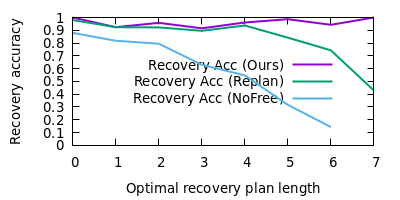
\includegraphics[width=0.9\textwidth]{figures/trend_errors.png}
       % \caption{(a}
       % \label{fig:graphs1}
    \end{subfigure}
    \begin{subfigure}{0.5\hsize}
       \centering    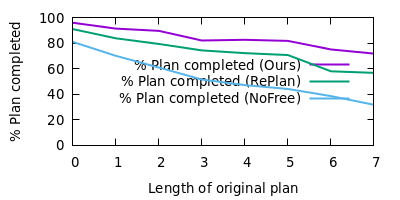
\includegraphics[width=0.9\textwidth]{figures/trend_steps.png}
       % \label{fig:graphs2}
    \end{subfigure}
    \caption{
        \footnotesize{
            Effect of complexity of errors and plan length on recovery accuracy and \% plans completed. %planning time (in sec)
        }
    }
    \label{fig:graphs}
    \vspace{-0.15in}
\end{figure}

\textbf{Simulation Results. }
Figure \ref{fig:rollout} demonstrates a 5-step instruction with an introduced error provided to a simulated 7-DOF Franka Emika manipulator in a table top setting. An external agent interchanges the location of 2 objects, which is detected using the predicted intermediate scene graph. A 3-step recovery plan is generated, which consists of first moving the yellow dice to a free space, followed by moving the two objects to their correct positions.

